\part{Bases de la programmation impérative et fonctionnelle}

Dans cette partie nous allons découvrir ce qu’est la programmation impérative et
fonctionnelle et acquérir les bases de l’algorithmie.

\chapter{Avant de commencer}

\section{Comment lire ce cours}
\subsection{Pré requis}
Pour profiter pleinement de ce cours, il faut :
\begin{itemize}
\item Disposer d'un Mac (récent) tournant sous OS X Yosemite (10.10).
\item Être \emph{persévérant}, \emph{rigoureux} et \emph{logique}.
\item Ne pas faire une allergie à la langue de Shakespeare (On croirais entendre mourir un
auvergnat, je sais ;).
\item Un petit bagage mathématique, de préférence niveau troisième, mais un collégien ayant
acquis le primaire devrait s'en sortir en s’accrochant un peu.
\end{itemize}

\subsection{De le méthode}
Ce cours essaye d'être accessible au débutant, mais il est important d'acquérir de bonnes
bases pour pouvoir comprendre la suite. Certains chapitres peuvent être très denses,
donc n'hésitez pas à les relire plusieurs fois.
Pour bien acquérir un cours, il faut :
\begin{description}
\item[Le Comprendre] car on ne peut pas retenir et appliquer un cours sans le comprendre.
\item[Le Reprendre] plusieurs fois, car une bonne mémorisation ne peut se faire qu'à ce prix.
\item[Le Pratiquer], c'est à dire ne pas copier coller bêtement mon code sans le comprendre.
C'est en cherchant que l'on tire le meilleur profit d'un exercice : Tiens, j'ai essayé ça,
Pourquoi cela n'a il pas marché ? Essayez d'être curieux, de pousser mes exemples
dans leurs retranchements, de les modifier. Ne jetez pas l'éponge si vous n'avez pas
d'idée après 5 secondes ou si votre première idée ne marche pas. Enfin, essayez
d'exécuter pas à pas votre code dans votre tête pour vérifier qu'il fait bien ce que vous
aviez l'intention de faire.
\end{description}
Cette méthode de travail est la \emph{meilleure}, d'expérience d'élève de classe prépa (NB cette
méthode marche à tous les niveaux).
\subsection{Risque d’évolution}
Ce cours est susceptible d'évoluer rapidement du fait que Swift n'est pas encore stabilisé.

Le site \url{https://github.com/ksm/SwiftInFlux/blob/master/README.md}  répertorie les
évolutions de Swift, y compris celles qui ne sont qu’envisagées.
\section{Quelques notions sur le fonctionnement d'un ordinateur}
\subsection{Qu'est-ce qu'un ordinateur ?}
Qu'est-ce qu'un ordinateur ? Avant tout une machine qui manipule des données (par
exemple la photo de votre chat, chien, petit-neveu ; le site Web que vous consultez, ou le
résultat d'une expérience du LHC), et cela selon un programme qui peut être changé,
c'est à dire que le programme est lui même une sorte de donnée.

Ainsi, les organes les plus importants d'un ordinateur sont sa mémoire et le processeur
qui exécute le programme, lui aussi stocké en mémoire.

Ensuite, un ordinateur possède aussi des entrées et des sorties, qui lui permettent de
communiquer avec le reste du monde (la carte graphique qui affiche ce texte à l'écran, la
carte réseau qui permet de charger des pages Web, la carte son, un clavier, une souris...).

Distinction supplémentaire : Un ordinateur possède 2 grands types de mémoire, une
mémoire qui ne s'efface pas si on coupe le courant, mais qui a généralement
l'inconvénient d'être lente, c'est par exemple le disque dur ou l'antique disquette ; et pour
pallier à cet inconvénient, un mémoire rapide, de moindre capacité et non persistante, la
mémoire vive ou RAM. Il y a aussi des mémoires dans lesquelles on ne peut que lire, qui
contiennent parfois les instructions nécessaire au démarrage de l'ordinateur.
\subsection{Qu'est-ce qu'un programme ?}
Un programme c'est la suite des instructions que doit exécuter le processeur
(e.g.\ additionner deux nombres, afficher bonjour à l'écran...).

Programmer, c'est créer un nouveau programme pour l'ordinateur.

Sauf qu'un ordinateur ne parle pas français, ni anglais, d'ailleurs ; Un ordinateur parle un
langage qui lui est propre, le \emph{binaire}, une suite de 0 et de 1, qui sont organisés en
instructions plutôt basiques, (par exemple écrit à tel emplacement dans la mémoire le
nombre 42, ou le résultat de l'addition de deux nombres en mémoire...). Ce n'est donc pas
raisonnable d'écrire un programme comme cela.
\section{Comment se faire comprendre d'un ordinateur ?}
\subsection{Un langage de programmation ?}
La première idée que l'on a eu c'est de mettre des mots un peu plus clair pour chaque
instruction, et d'utiliser un programme, l'\emph{assembleur}, pour effectuer la traduction. C'était
mieux, mais pour écrire du texte a l'écran et faire de jolis boutons, c'était encore trop
difficile.
\begin{listing}[H]
\caption{Exemple d'assembleur x86\_64, tiré de Qt}
\begin{minted}[linenos=true]{asm}
q_atomic_increment:
	lock
	incl (%rdi)
	setne %al
	ret
	.size q_atomic_increment,.-q_atomic_increment

	.globl q_atomic_decrement
        .type q_atomic_decrement,@function
        .section .text, "ax"
        .align 16
\end{minted}
\end{listing}

C'est pour cela que l'on a inventé d'autres langages de programmation, de plus en plus
élaborés, qui sont ensuite traduits par un autre programme en code binaire.

L'un des langage ayant marqué l'informatique est le langage \emph{C}.

On classe donc les langages selon leur niveau d'abstraction par rapport au
fonctionnement de l'ordinateur. L'\emph{assembleur} est un langage de bas niveau, très (trop)
prohe du fonctionnement du processeur, tandis que le \emph{C} est de haut niveau (permettant
d'ordonner au processeur beaucoup de choses en une instruction), et le \emph{python},de très
haut niveau, pour ne citer que quelques exemples d'une très longue liste.%Liste Wiki

\emph{Swift}, le langage que nous allons étudier, est un langage de plus haut niveau
que le C.
\subsection{Swift}
Swift a été développé au sein d'Apple, sous l'égide de Chris Lattner à partir de 2010, et a
été présenté au monde en juillet 2014. Ce langage se veut << \emph{l'Objective-C sans le C} >>.

L'\emph{Objective-C} était le langage utilisé par Apple jusque là, mais qui était une extension du
C, ce qui impliquait que langage restait limité par la gestion de mémoire du C délicate et propre à causer de erreurs et failles de sécurités.

Le but était de créer un langage puissant, rapide, et sécurisé, mais avec une syntaxe
aussi agréable à utiliser qu’un langage de script.
\section{Les outils du programmeur}
Si vous avez bien lu la partie précédente, vous devriez déjà en avoir identifié un.

Il s'agit (comme vous l'avez tous deviné) d'un programme qui traduit notre code en
langage de haut niveau, appelé \emph{code source}, en code binaire. On l'appelle le
\emph{compilateur}.


Le deuxième outil est celui qui permet d'éditer le code (les plus malins m'auront vu venir).

Comme le code s'écrit dans des fichiers textes, un simple éditeur de texte, comme
TextEdit, pourrait suffire. Cependant les programmeurs utilisent en général des éditeurs
dédiés qui possèdent des fonctionnalités supplémentaires, comme la coloration du code.
% (cf Illustration en page suivante, il s’agit de l’éditeur TextWrangler)

Enfin un troisième outil est un debugger, qui permet de contrôler l'exécution pas à pas du
programme, pour comprendre pourquoi ça ne marche pas. (En théorie, si l'on ne faisait
pas d'erreur on pourrait s'en passer, mais << \emph{errare humanum est.} >> )

Mais pour simplifier les choses, il a été créé un type de programme particulier, les \emph{IDE,
Environnements de Développement Intégrés}, qui regroupent ces trois fonctionnalités. Sur
Mac OS X, cet EDI s'appelle \emph{Xcode}, et nous l'allons installer tout à l'heure !
\chapter{Découvrons XCode}
Dans cette parte nous allons installer et découvrir l'IDE d’Apple, puis découvrir notre
première ligne de code.
\section{Installation de XCode}
L'installation de cet outil est plutôt facile, puisqu’il est disponible depuis le Mac app Store,
gratuitement. On peux aussi le télécharger depuis le site des développeurs Apple. Il faut
cependant s'inscrire en tant que développeur avec son Apple ID, gratuitement, pour
accéder aux divers ressource, dont la documentation,
je vous recommande donc de le faire.
(Attention , les programmes payants ne sont pas nécessaires, il servent juste à pouvoir
soumettre des applications sur les App Store, et pouvoir signer son code, pour la
distribution via internet)
Une fois les quelques Giga-octets de l'application téléchargés (grosse pause café), vous
verrez l'application apparaitre dans votre dossier application.
\begin{figure}[h]
\centering
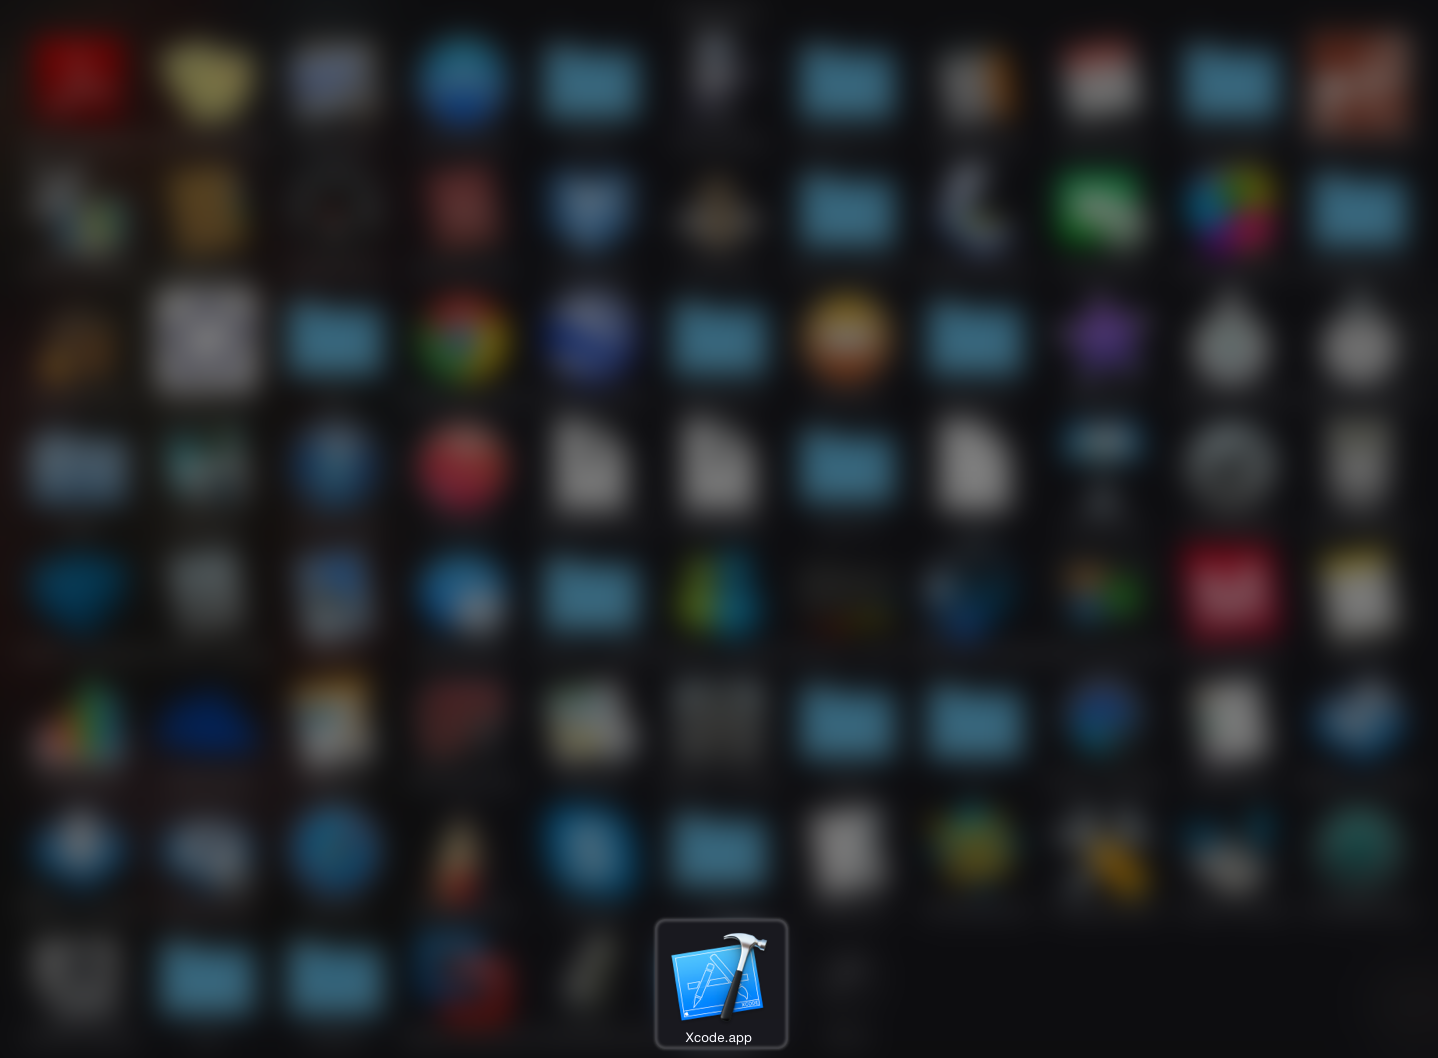
\includegraphics[scale=0.30]{\TSwiftRoot/P1/CH2/img/Launchpad}
\caption{L'icône de XCode dans la pile Applications}
\end{figure}

\section{Premier contact avec Swift, un Playground}
Ouvrez XCode. Vous devez voir apparaitre cette fenêtre, à la colonne de droite près.
\begin{figure}[h]
\centering
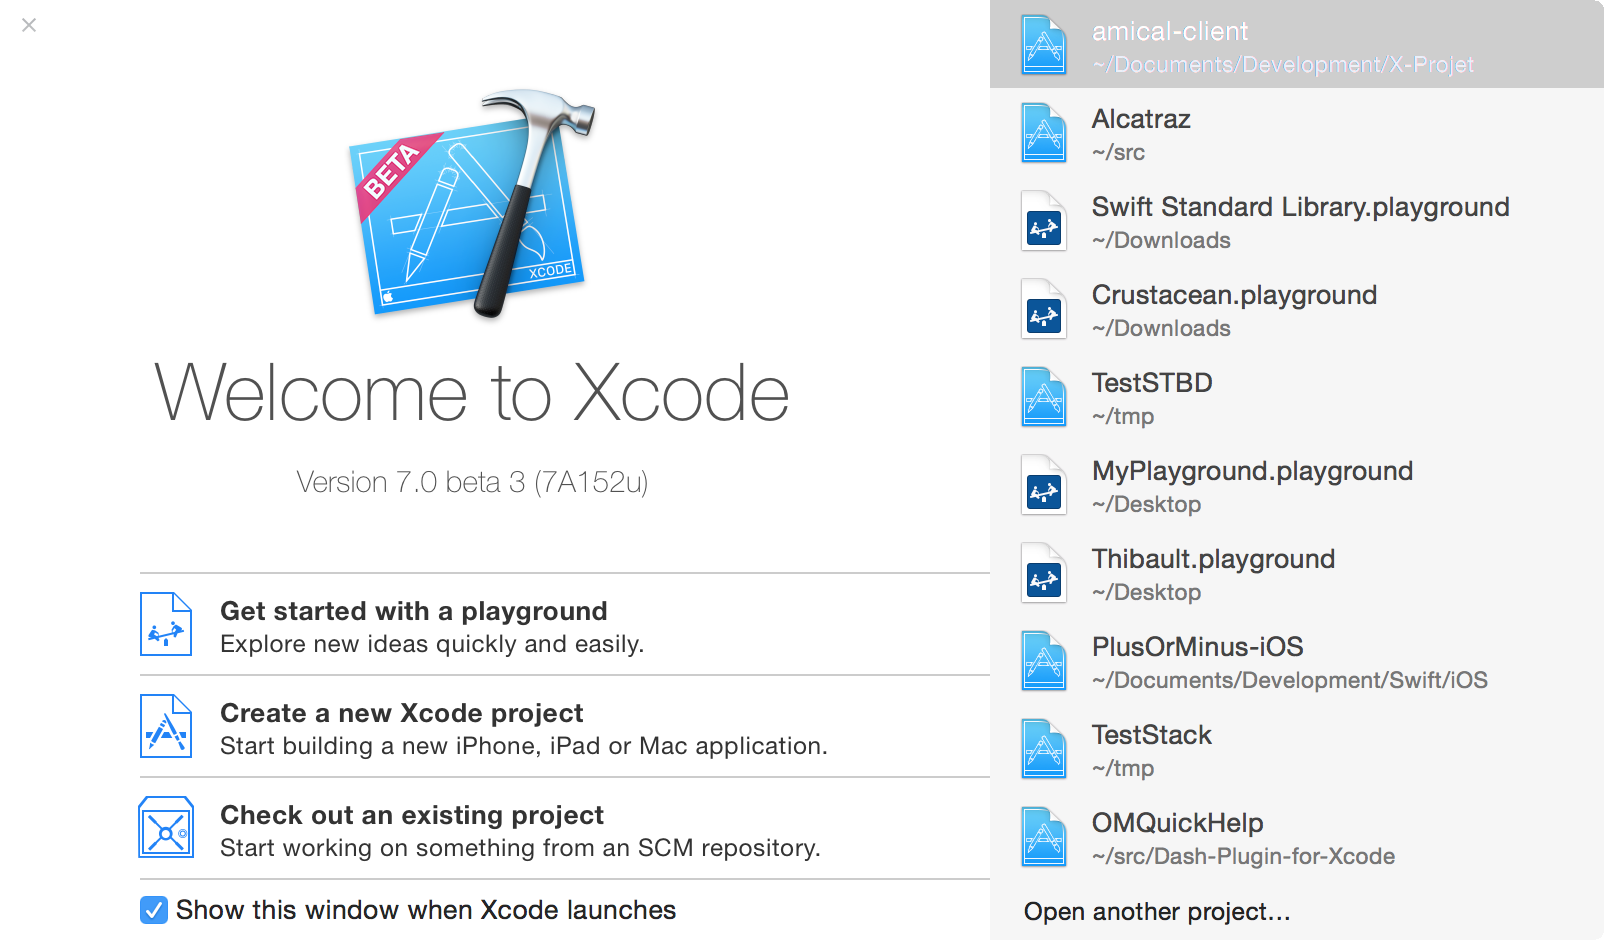
\includegraphics[scale=0.5]{\TSwiftRoot/P1/CH2/img/XCodeWindow}
\caption{Fenêtre d'accueil de XCode}
\end{figure}

Cliquez sur << Get started with a playground >>, pour créer un nouveau playground.
Choisissez comme plateforme OS X, et donnez lui un nom sensé.
Une fois le projet enregistré, vous voyez apparaitre une fenêtre en deux parties.
A gauche un éditeur de texte qui contient du code Swift, à droite une colonne dans
laquelle sont affichés les résultats de chaque instructions.
En Swift une instruction se termine par un retour à la ligne, ou un point virgule (Si on tient
absolument à mettre plusieurs instructions sur une ligne).
Vous avez normalement le code suivant, affichant \verb"Hello, playground" en face de la troisième ligne :
\begin{listing}[h]
\caption{Code par défaut d'un Playground Swift}
\begin{minted}[linenos=true]{swift}
// Playground - noun: a place where people can play

import Cocoa

var str = "Hello, playground"
\end{minted}
\end{listing}

Remplacez le par le code suivant :
\begin{listing}[h]
\caption{Programme affichant "Hello, playground"}
\begin{minted}[linenos=true]{swift}
// Playground - noun: a place where people can play

println("Hello, playground")
\end{minted}
\end{listing}

Ce code semble avoir le même effet que le précédent, mais cela n'est vrai que dans un playground, qui est un environnement très particulier.

Il s’agit du premier programme que l’on montre par convention dans un nouveau langage :
« Hello, World ! », qui affiche à l’écran le texte en question.

La première ligne de code est un commentaire (ignoré royalement par le compilateur)
notion que nous étudieront dans la prochaine section, la deuxième la ligne qui affiche le
texte << Hello, Playground ! >> (sans les guillemets à l’écran).
On reviendra plus en détail sur cette ligne plus tard, mais je tenait à vous présenter ce
programme, qui est plutôt court dans ce langage (1 ligne en Swift, contre 4 lignes en C).

Vous pouvez remplacer le texte entre guillemet par le texte que vous voulez.

\mintinline{swift}{println} est la fonction qui est chargé d’afficher à l’écran une ligne de texte.

Cette ligne de code correspond à une \emph{instruction}.
Il est possible de mettre \emph{plusieurs} instructions par lignes à condition de laes séparer par des points virgule\verb";".

Un playground est un outil très puissant de XCode puisqu’il permet de voir immédiatement
les conséquences d’une modification du code.
\section{Les Commentaires}
Un commentaire permet à l’auteur du code d’expliquer ce qu’il fait, ou plus généralement
d’introduire dans le code source du texte ignoré par le compilateur.

Vous allez me dire, que vous ne voyez pas à quoi cela sert. En fait, lire le code d’un autre
programmeur n’est pas toujours évident, (à quoi ça sert ça !? Et qu’est ce que tu veux faire
là ?). Pour aider les autres, et soi même, lorsqu’on se replonge dans son code des mois après, il est donc
indispensable d’expliquer son code.

Comme un court exemple vaut mieux qu’un long discours je vous laisse consulter le code.

\emph{Attention à ceux qui connaissent les commentaires du C, en Swift, les commentaires
s'imbriquent les un dans les autres.}

\begin{listing}[h]
\caption{Que de commentaires !}
\begin{minted}[linenos=true]{swift}
// Ceci est un commentaire s'arrêtant en fin de ligne.
/* Ceci est un commentaire qui s'arrête au symbole */
/*
Il peut s'étendre sur plusieurs lignes
// Je suis un commentaire imbriqué
/*Moi aussi*/
println("Hello, playground")
Mais rien ne se passe !
Fin du commentaire sur plusieurs lignes:*/
// On peut placer un commentaire après une instruction
println("Hello, playground") // Comme ici.
// Ou même au milieu
println(/*Texte ici*/"Bonjour, bac à sable") // Parce qu'en Français c'est mieux.
\end{minted}
\end{listing}
Remarquez que XCode colore les commentaires d'une couleur particulière (chez moi, le vert).
\section{Un quasi-interpréteur : La REPL Swift}
Le playground, est un outil très puissant puisqu’il compile et exécute immédiatement
chacune de vos instructions.

En arrière plan, XCode compile automatiquement votre programme, et utilise le debugger
pour obtenir l’état du programme après chaque instruction.

Il existe une autre façon de jouer avec Swift, un peu moins jolie mais encore plus rapide
qu’un playground qui reste un fichier : La << Read Eval Print Loop >>, boucle de lecture évaluation écriture, basé elle aussi sur le
débugger. Si vous avez déjà utilisé la ligne de commande ou utilisé un langage interprété
comme Python, je vous la présente ici, sinon vous pouvez sauter cette partie, ou vous
référer au tutoriel OSX ici \url{http://openclassrooms.com/courses/domptez-votre-mac-avec-os-x-yosemite/le-terminal-dans-os-x-1}.

Ouvrez un Terminal Unix, et tapez \verb"swift".
Tapez ensuite une ligne de code et appuyez sur entrée.
swift affiche alors le résultat.
Pour quitter tapez \verb":quit".
En arrière plan Swift compile la ligne de code puis l'exécute et affiche le résultat.
Attention, contrairement à un interpréteur qui lit la ligne dans son langage et exécute
les instructions en question, il y a bien ici création du code binaire correspondant.
Cet outil peut être très puissant, mais je ne le détaillerai pas ici, libre à vous de l’explorer.
\begin{listing}[h]
\caption{Exemple de sortie après un usage de la REPL Swift}
\begin{verbatim}
$ swift
Welcome to Swift!  Type :help for assistance.
  1> println("Hello, REPL")
Hello, REPL
  2> :quit
$
\end{verbatim}
% Check if this is correct.
\end{listing}
\chapter{Les variables, les constantes, un peu d'arithmétique}
Comme je l'ai dit, un ordinateur manipule des données. Il faut donc pouvoir les stocker
quelque part.
\section{La mémoire d'un ordinateur, qu'est-ce qu'une \emph{variable} ?}
Une \emph{variable}, c'est avant tout un compartiment de la mémoire de l'ordinateur sur lequel on colle un nom, et dans lequel on a le droit de mettre ce que l'on veut, pour pouvoir y accéder ultérieurement.

L'unité de base de la mémoire d'un ordinateur est \emph{le} bit (pas la !), qui possède deux états,
1 ou 0, à comparer aux 10 chiffres de notre système décimal.

Pour stocker des nombres
plus grand, il faut mettre plusieurs bits cote à cote, comme nous mettons plusieurs chiffres
pour écrire 1999, par exemple. Dans ce cas, le dernier chiffre correspond aux unités, l'avant dernier à
des paquets de 2, l'antépénultième 4, ... 8, 16, 32, 64... .

Les bits sont regroupés en mots
appelés \emph{bytes} en anglais, d'une taille fixée par l'architecture du processeur. En français
on traduit improprement ce terme par octet, qui désigne un mot/byte de 8 bit qui peut prendre
\begin{math}2*2*2...*2\end{math} huit fois, noté \begin{math} 2^{8} \end{math}. Soit 256 valeurs (retenez ce nombre, on le retrouvera par la suite.)
Toute la mémoire est découpé en bytes. On manipule forcément un ensemble de byte. (1,
2, 4, ...), et donc toute variable a une taille définie qui est un multiple de l'octet.

L'ordinateur peut aussi stocker des nombres binaires à virgule, comme nos nombres à virgule, avec les limitations de ces derniers. Je ne détaille pas ici toute la représentation, si vous voulez des details je vous renvoie à cet excellent tutoriel :

\url{http://openclassrooms.com/courses/fonctionnement-d-un-ordinateur-depuis-zero}

\emph{Mais il n'y a que des nombres, comment on stocke du texte ?!}
Désolé, mais pour l'ordinateur, tout est un nombre, tout dépend de la façon dont on
l'interprète, on y viendra un peu plus tard.
\section{Demander poliment de la place pour stocker un nombre}
Passons à la pratique !
\subsection{Déclarons l'age du Capitaine}
\begin{listing}[h]
\caption{Premier exemple, l'age du Capitaine}
\begin{minted}[linenos=true]{swift}
var age_du_capitaine = 42 // ;-)
\end{minted}
\end{listing}
Décortiquons ce qui précède :
\begin{description}
\item[var :] Mot \emph{clé} indiquant que l'on veut déclarer une variable.
\item[age\_du\_capitaine :] Nom de la variable, qui nous permettra d'y accéder de nouveau. \emph{Attention, il ne peut pas y avoir deux variables de même nom}
\item[= :] Opérateur utilisé pour doner une valeur à une variable.
\item[42 :] La valeur entière que l'on donne à notre variable.
\item[// ;-) :] C'est un commentaire. Si vous ne le saviez pas, \emph{relisez le chapitre précédent}.
\end{description}
\subsection{Différents types d'entiers}
Je vous ai parlé de la représentation en mémoire des entiers, donc vous devriez me demander comment Swift détermine le nombres d'octets qui sont attribués à notre entier. La réponse c'est qu'il a attend qu'on  le lui précise, ou il prend une valeur par défaut.
Il existe donc plusieurs type d'entiers, chacun pouvant contenir une plage de nombre particulière. Notamment, il existe des variantes non signées, qui ne contienne que des nombres positifs.

\begin{longtabu} to \linewidth {|X[3,l,m]|X[1.5,l,m]|X[6,r,m]|X[1,r,m]|}
\hline Taille & Type & Plage de valeur & Précision \\ \hline
\endhead
Architecture (32 ou 64 bits) & \mintinline{swift}{Int} (par défaut) & 32 bits : \mintinline{swift}{Int32}, 64 bits : \mintinline{swift}{Int64} & 1 \\ \hline
Architecture (32 ou 64 bits) & \mintinline{swift}{UInt} & 32 bits : \mintinline{swift}{UInt32}, 64 bits : \mintinline{swift}{UInt64} & 1 \\ \hline
1 octet soit 8 bits & \mintinline{swift}{Int8} & -128 à 127 & 1 \\ \hline
1 octet soit 8 bits & \mintinline{swift}{UInt8} & 0 à 255 & 1 \\ \hline
2 octets soit 16 bits & \mintinline{swift}{Int16} & -32768 à 32767 & 1 \\ \hline
2 octets soit 16 bits & \mintinline{swift}{UInt16} & 0 à 65535 & 1 \\ \hline
4 octets soit 32 bits & \mintinline{swift}{Int32} & -2147483648 à 2147483647 & 1 \\ \hline
4 octets soit 32 bits & \mintinline{swift}{UInt32} & 0 à 4294967295 & 1 \\ \hline
8 octets soit 64 bits & \mintinline{swift}{Int64} & -9223372036854775808 à 9223372036854775807 & 1 \\ \hline
8 octets soit 64 bits & \mintinline{swift}{UInt64} & 0 à 18446744073709551615 & 1 \\ \hline

\caption{Les différents Types d'entiers}
\end{longtabu}

Attention, n'essayez pas de mélanger des types différents ou le compilateur vous fera amèrement regretter. On discutera de ce problème un peu plus en détail dans la quatrième section.

Par exemple pour déclarer que l'on stocke l'age du Capitaine sur 1 octet (soit 8 bit) et que ce doit être un entier non signé (positif) on utilise :

\begin{listing}[h]
\caption{Un type plus approprié pour l'age du capitaine}
\begin{minted}[linenos]{swift}
var age_du_pitaine : UInt8  = 42 // Question ? Quel est l'age maximal du capitaine
\end{minted}
\end{listing}
Le caractère \verb":" permet d'introduire une \emph{annotation de type}, tandis que \verb"UInt8" correspond au type d'entier choisi.

Remarquez que Swift est ici plutôt agréable à utiliser puisqu'il ne nous oblige pas à lui préciser le type lorsque la réponse est évidente, mais nous permet d'être plus précis si on en a besoin.
\subsection{La structure générale}
La structure générale est la suivante, ou les parties entre crochets peuvent être absente, mais pas toute les deux.
\begin{listing}[h]
\begin{minted}[linenos]{swift}
var <nom de variable> [ : <Type> ] [ = <valeur initiale> ]
\end{minted}
\caption{Structure générale d'une déclaration de variable}
\end{listing}
\begin{description}
\item[nom de variable :] Un nom de variable peut être composé de n'importe quel caractère unicode à part les espaces, les flèches et symboles mathématiques et les caractères Unicode invalides ou servant à dessiner des lignes et des boites, soit à peu près tout ce que vous puvez vouloir utiliser. Il ne doit pas commencer par un chiffre.
\item[Type :] Il peut être omis si une valeur initiale est précisée, permettant à Swift de déduire le Type.
Le mot clé \mintinline{swift}{typealias} permet de définir un type comme étant la même chose qu'un type déja existant (Les noms de types suivent les même règles que les noms de variable). Exemple \mint{swift}|typealias Age = UInt8|
\emph{Toute variable possède un type.}
\item[valeur initiale :] Il est recommandé d'initialiser une variable à sa déclaration, mais ce n'est pas obligatoire, dans ce cas il est indispensable de préciser le type pour que Swift s'y retrouve. Dans ce cas il faut aussi garantir que la variable sera toujours initialisée avant d'y accéder pour la première fois, sinon le programme ne compilera pas.
\end{description}
Il est possible de déclarer plusieurs variables en même temps, exemple :
\mint{swift}|var frères = 5, sœurs = 4 // c'est une famille nombreuse !|
\subsection{Les nombres à virgule flottante}
Parlons maintenant des nombres à virgule (ou à points, puisque tel est le séparateur décimal en Angleterre et donc dans le monde des programmeurs).
Ces nombres ont un défaut, il ne peuvent pas représenter parfaitement tous les nombres décimaux, comme un nombre décimal ne peu pas représenter parfaitement \begin{math} \frac{1}{7} \end{math}, par exemple. Mais en général cette approximation n'est pas un problème.
Il y deux principaux types de nombres à virgule, ainsi qu'un troisième, moins commun, que je cite par soucis d'exhaustivité :
\begin{longtabu} to \linewidth {|X[3,l,m]|X[1,l,m]|X[4,r,m]|X[3,r,m]|}
\hline Taille & Type & Plage de valeur (approximative) & Précision \\ \hline
\endhead
4 octets soit 32 bits & \mintinline{swift}{Float} & \begin{math}\pm10^{-38}\end{math} à \begin{math}\pm10^{-38}\end{math} & 6 chiffres décimaux \\ \hline % Vérifier la précision.
8 octets soit 64 bits & \mintinline{swift}{Double} & \begin{math}\pm10^{-308}\end{math} à \begin{math}\pm10^{308}\end{math} & 15 chiffres décimaux \\ \hline
10 octets soit 80 bits & \mintinline{swift}{Float80} & \begin{math}\pm 3.65×10^{−4951}\end{math} à \begin{math}\pm1.18×10^{4932}\end{math} & 18 chiffres décimaux \\ \hline

\caption{Les différents Types de nombres à virgule flottante}
\end{longtabu}

\subsection{Changer la valeur d'une variable}
Pour changer la valeur d'une variable il suffit d'utiliser l'opérateur \verb"=".
\begin{listing}[h]
\caption{Un type plus approprié pour l'age du capitaine}
\begin{minted}[linenos]{swift}
var sens_de_la_vie = 5 // Int
sens_de_la_vie = 42 // Parce que c'est la seule bonne réponse !
var six_fois_sept = sens_de_la_vie // ça marche aussi.
var pi = 3.14 // Double
pi = 3.141592 // Plus précis !
\end{minted}
\end{listing}

\emph{Attention, on ne peut pas changer le type d'une variable après qu'elle est été défini.}
\subsection{Récapitulatif des types de nombres}
\begin{longtabu} to \linewidth {|X[2,l,m]|X[1,l,m]|X[4,r,m]|X[2,r,m]|}
\hline Taille & Type & Plage de valeur (approximative) & Précision \\ \hline
\endhead
Architecture (32 ou 64 bits) & \mintinline{swift}{Int} (par défaut) & 32 bits : \mintinline{swift}{Int32}, 64 bits : \mintinline{swift}{Int64} & 1 \\ \hline
Architecture (32 ou 64 bits) & \mintinline{swift}{UInt} & 32 bits : \mintinline{swift}{UInt32}, 64 bits : \mintinline{swift}{UInt64} & 1 \\ \hline
1 octet soit 8 bits & \mintinline{swift}{Int8} & -128 à 127 & 1 \\ \hline
1 octet soit 8 bits & \mintinline{swift}{UInt8} & 0 à 255 & 1 \\ \hline
2 octets soit 16 bits & \mintinline{swift}{Int16} & -32768 à 32767 & 1 \\ \hline
2 octets soit 16 bits & \mintinline{swift}{UInt16} & 0 à 65535 & 1 \\ \hline
4 octets soit 32 bits & \mintinline{swift}{Int32} & -2147483648 à 2147483647 & 1 \\ \hline
4 octets soit 32 bits & \mintinline{swift}{UInt32} & 0 à 4294967295 & 1 \\ \hline
8 octets soit 64 bits & \mintinline{swift}{Int64} & -9223372036854775808 à 9223372036854775807 & 1 \\ \hline
8 octets soit 64 bits & \mintinline{swift}{UInt64} & 0 à 18446744073709551615 & 1 \\ \hline

4 octets soit 32 bits & \mintinline{swift}{Float} & \begin{math}\pm10^{-38}\end{math} à \begin{math}\pm10^{-38}\end{math} & 6 chiffres décimaux \\ \hline % Vérifier la précision.
8 octets soit 64 bits & \mintinline{swift}{Double} & \begin{math}\pm10^{-308}\end{math} à \begin{math}\pm10^{308}\end{math} & 15 chiffres décimaux \\ \hline
10 octets soit 80 bits & \mintinline{swift}{Float80} & \begin{math}\pm 3.65×10^{−4951}\end{math} à \begin{math}\pm1.18×10^{4932}\end{math} & 18 chiffres décimaux \\ \hline

\caption{Les différents types de nombres}
\end{longtabu}
Notez aussi que les nombres littéraux, que vous tapez n'ont pas de type a priori, et que le type résultant n'est déterminé qu'après comme étant Int ou Double, si le résultat n'est pas entier. Il existe plusieurs notations(décimale, hexadécimale, octale, binaire), mais je ne vous les présente pas ici.
\section{Variables et Constantes}
On peut en fait imposer que la valeur d'une variable ne change plus après sa création :
c'est alors une constante. Elle se déclare comme une variable excepté que l'on utilise le
mot clé \mintinline{swift}{let}, et que sa valeur doit être fixé à la déclaration, dans ce cas toute tentative de changement de la valeur résulte en une erreur à la compilation.
\begin{listing}[h]
\begin{minted}[linenos=true]{swift}
let pi = 3.141592
// Que personne n'essaye de changer pi !
pi = 3.1416 // Erreur !
\end{minted}
\end{listing}

Du fait de cette déclaration, le compilateur peut d'une part vous prémunir d'une erreur, et
d'autre part réaliser des optimisations supplémentaires. Apple vous recommande d'utiliser
des constantes en priorité, et de ne déclarer comme variable que ce qui doit l'être.
\section{Une vraie calculatrice !}
Je l'ai déjà dit, mais un ordinateur n'est qu'une grosse calculatrice, et pour vous prouver que
je ne vous mène pas en bateau, nous allons nous en servir :
\subsection{Additionnons deux nombres}
Pour additionner deux nombres, on utilise l'opérateur plus, comme au primaire.
\begin{listing}
\begin{minted}[linenos]{swift}
let nombre1 = 64
let nombre2 = 36
let résultat = nombre1 + nombre2
// On initialise la constante résultat avec le résultat de l'addition des deux nombres.
let flottant = 1.5
let entier = 5
let resultat2 = flottant + Double(entier) // Conversion !
let pi = 3 + 0.141592 
// Ceci ne marche que parce que les nombres littéraux n'ont pas de type.
\end{minted}
\caption{Des additions}
\end{listing}

Attention, toutefois, au mélange des types. Pour additionner un entier et un nombre à virgule flottante il faut convertir  
\subsection{Soustraction et multiplication}
De même les bonnes vielles soustractions et multiplications fonctionnent, avec les mêmes règles de priorité des opérations en utilisant respectivement les opérateurs \verb"-" et \verb"*".
Exemple :
\begin{listing}
\begin{minted}[linenos]{swift}
let nombre1 = 10 * 10
let nombre2 = 6 * 6
let résultat = nombre1 - nombre2
// Pythagore à encore frappé. 
\end{minted}
\caption{Multiplications et Soustractions}
\end{listing}

\subsection{Division et modulo}
La division, vous connaissez, mais vous allez surment me demander ce que j'entends par \emph{modulo}.

Il s'agit en fait du nom que les programmeurs donnent au \emph{reste} de la division euclidienne.

Commençons par la division.

Il est possible de diviser deux entiers pour obtenir un eniter, et deux nombres à virgule pour obtenir un nombre à virgule, attention, les trois du même type, à vous de faire des conversiuons si besoin est : \mintinline{swift}{LeBonType(<var_du_mauvais_type>) + var_du_bon_type}.
\begin{listing}[h]
\begin{minted}[linenos]{swift}
let entier = 49
let flottant = 5.0
let quotient_entier = entier / Int(flottant)
// Division d'entier : 9
let quotient_flottant = Double(entier) / flottant
// Division de flottants : 9.8
\end{minted}
\caption{Les deux divisions}
\end{listing}

Le modulo \mintinline{swift}{(a % b)} est défini tel que \mintinline{swift}{a = b * un_entier + (a % b)} ou \verb"un_entier" est le plus grand entier en valeur absolue (en ommetant le signe) tel que \verb"a % b" soit du signe de \verb"a". \verb"a % b", est donc, en valeur absolue (sans le signe), strictement plus petit que \verb"b".
(en supposant b, positif, mais s'il est négatif on a le même réultat que s'il était positif)

En Swift, contrairement à la plupart des langage, le modulo n'est pas réservé à deux entiers, il est aussi possibel de l'appliquer à \emph{deux} nombres à virgule.

\begin{listing}[h]
\begin{minted}[linenos]{swift}
let entier = 49
let flottant = 5.0
let reste_entier = entier % Int(flottant)
// Division d'entier : 4
let reste_flottant = Double(entier) % 2.5
// Division de flottants : 1.5
\end{minted}
\caption{Le modulo, avec des entiers ou des flottants.}
\end{listing}

\subsection{Opérateurs augmentés}
J'avais aussi omis de vous le préciser, mais la qualité première du programmeur est la fainéantise. En fait je plaisante un peu, mais les programmeurs apprécient dès qu'ils ont moins à taper.
Par conséquent au lieu d'écrire \mintinline{swift}{a = a + 1}
Ils utilisent une notation raccourcis spéciale \mintinline{swift}{a += 1}

On appel ces opérateurs \emph{augmentés}. Ils existent pour les 5 opérateurs que nous avons déja vu :

\begin{longtabu} to \linewidth {|X[,l,m]|X[,l,m]|}
\hline Opérateurs augmenté & Opérateurs normal \\ \hline
\endhead
\mintinline{swift}{a += 1} & \mintinline{swift}{a = a + 1} \\ \hline
\mintinline{swift}{a -= 1} & \mintinline{swift}{a = a - 1} \\ \hline
\mintinline{swift}{a *= 2} & \mintinline{swift}{a = a * 2} \\ \hline
\mintinline{swift}{a /= 2} & \mintinline{swift}{a = a / 2} \\ \hline
\mintinline{swift}{a \%= 2} & \mintinline{swift}{a = a \% 2} \\ \hline
\caption{Les différents opérateurs augmentés}
\end{longtabu}

\subsection{Incrémenter et Décrémenter}
Comme les programmeurs sont vraiments très fainéants il existe deux opérateurs pour ajouter et enlever 1 à une variable : \mintinline{swift}{++} et \mintinline{swift}{--}, formes raccourcies respectives de \mintinline{swift}{+=1} et \mintinline{swift}{-=1}. Ils peuvent être placés avant ou après une variable, avec une légère différence en terme de priorité, dont nous parlerons dans le chapitre dédié aux opérateurs avancés.
\section{Première approche des fonctions}
Vous vous souvenez de la ligne affichant du texte, au chapitre 2. Je vais ici vous l'expliquer un peu plus en détail.
\subsection{Une fonction}
Pour le matheux : \emph{Une fonction associe à tout élément d'un ensemble de départ au plus un élément d'un ensemble d'arrivé}.

Pour le programmeur, une fonction c'est donc une sorte de boite noire, à laquelle on donne à manger des paramètres, \emph{de types bien définis}, et qui renvoi une valeur (ou rien du tout).

Une fonction sert à réutiliser un bout de code sans avoir à le recopier à chaque fois, et permet de ne pas avoir à savoir comment cela fonctionne.
On reviendra à l'utilité du découpage du code dans un chapitre ultérieur.

L'exemple que vous avez déja vu est la fonction \mintinline{swift}{println}, qui affiche une ligne de texte. Les conversion de type sont aussi à des fonctions.

\begin{listing}[h]
\begin{minted}[linenos]{swift}
let entier = 42
let flottant = Double(entier)
println("Bonjour tout le monde")
\end{minted}
\caption{Deux appels de fonctions}
\end{listing}

Un appel de fonction se présente sous la forme :
\pagebreak % Required hack, because if not some texts disapears out of the page.
\begin{listing}[h]
\begin{minted}[linenos]{swift}
nom_de_la_fonction(<paramètre>[, <paramètre2 ...]) 
\end{minted}
\caption{forme générale d'un appel de fonction}
\end{listing}

Ici les noms correspondants sont \mintinline{swift}{Double} (le nom du type, en effet ...) et \mintinline{swift}{println}. La deuxième ne renvoie rien, tandis que la première renvoie un \mintinline{swift}{Double} (comme c'est original ...), que l'on récupère ici dans une variable, mais qui aurait pu être utilisé dans une autre expression, comme paramètre d'une autre fonction, ou dans une opération.

\subsection{Les Fonctions mathématiques}

Pour ceux qui connaissent un peu les maths, je vais ici vous donner la liste des fonctions disponibles dans Swift. Attention, ce ne sont pas de vraies fonctions au sens mathématiques, donc pas de dérivation, intégration, limite et autres.
\begin{description}
\item[pow :] La fonction puissance, prend deux paramètre Double ou Float $x$ et $a$, et renvoie $x^{a}$. % Penser à faire un TP Opérateur **
\item[abs :] Cette bonne vieille fonction valeur absolue (Int et Double).
\item[exp :] L'exponentielle d'un Double

J'en passe et des meilleurs, dont les fonctions trigonométriques (ainsi qu'inverses et hyperboliques, logarithmes...)
\end{description}
\chapter{Première approche des chaînes de caractères}
Dans ce chapitre, nous allons découvrir le type \mintinline{swift}{String}, de terme anglais pour ficelle, et qui n'a (cachez votre déception !) rien à voir avec un maillot de bain.

Il s'agit du type permettant de stocker de chaînes de caractères. Pour information, chaque caractère correspond à un nombre dans la mémoire de l'ordinateur, mais comme Swift utilise l'Unicode (qui permet de coder n'importe quel caractère informatique existant) le détail du fonctionnent des chaines de caractère est extrêmement complexe, et je ne le détaillerai pas ici !
\section{Playground, dis bonjour au monsieur}
Pour introduire une chaîne de caractère littérale dans votre code, il suffit d'écrire votre texte entre des guillemets doubles \verb'"', une variable ou constante se déclarant exactement de la même manière :
\begin{listing}[h]
\begin{minted}[linenos]{swift}
let bonjour = "Bonjour tout le monde !"
let au_revoir = "J'espère avoir le plaisir de vous revoir"
\end{minted}
\end{listing}
Pour insérer certains caractères spéciaux, interprétés par Swift de façon spécifique, par exemple, comme fin de chaîne il est nécessaire d'utiliser le caractère \verb"\".
% Tableau récap.
\begin{longtabu} to \linewidth {|X[1,l,m]|X[4,l,m]|}
\hline
Séquence & Signification \\ \hline
\endhead
% à vérifier
% Source : C99 last draft.
\verb"\\" & Permet d'insérer un \verb"\" sans qu'il soit interprété. \\ \hline
\verb"\0" & Caractère nul. Utilisé en C pour marquer la fin d'une chaîne ; en Swift, il est simplement ignoré. \\ \hline
\verb"\n" & Nouvelle ligne (Unix). \\ \hline
\verb"\r" & Retour chariot (Utilisé sur d'autres systèmes). \\ \hline
\verb"\t" & Tabulation horizontale. \\ \hline
\verb'\"' & Guillemet double : \verb'"'. \\ \hline
\verb"\'" & Guillemet simple : \verb"'". \\ \hline
\verb"\u{n}" & Caractère Unicode arbitraire de code hexadécimal $n$. \\ \hline

%\caption{Les caractères spéciaux}
\end{longtabu}

Je vous passe les détails sur l'Unicode. Pour les curieux je vous renvoie à la doc : \url{https://developer.apple.com/library/prerelease/ios/documentation/Swift/Conceptual/Swift_Programming_Language/StringsAndCharacters.html#//apple_ref/doc/uid/TP40014097-CH7-ID285}

Un élément d'une chaîne de caractère est un caractère, de type \mintinline{swift}{Character}, très difficile à distinguer d'une chaîne de caractère de longueur 1, à ceci près qu'on ne peut pas la rallonger.
\section{Concaténer deux chaînes}
Il est possible de créer une chaîne en mettant bout à bout deux (voir plusieurs) chaînes ou carctères, on dit alors que l'on \emph{concatène} ces chaînes. En Swift, l'opérateur \verb"+", que l'on a déja croisé, permet aussi de concaténer deux chaînes de caractères.

De même étant donné une variable \mintinline{swift}{String} déja existante, on peut lui concaténer une seconde chaîne en utilisant \verb"+=".
Ceci ne peux être fait avec une variable de type \mintinline{swift}{Character}
Exemple :
\begin{listing}[h]
\begin{minted}[linenos]{swift}
let bonjour = "Bonjour tout le monde !"
let au_revoir = "J'espère avoir le plaisir de vous revoir"
var discussion = bonjour + " ... " + au_revoir
// Notez les espaces dans la chaîne
// On a oublié le point !
discussion += "."
\end{minted}
\end{listing}
\section{Insérer la valeur d'une variable dans une chaîne de caractères}
Il est possible d'insérer la valeur d'une variable dans une chaine de caractère (sous réserve que son type le permette), ce qu'Apple appelle interpolation dans une chaîne de caractères, en utilisant la syntaxe suivante :
\begin{listing}[h]
\begin{minted}[linenos]{swift}
var str = "La variable contient \(nom_de_la_variable)"
\end{minted}
\caption{Interpolation dans une chaine de caractères.}
\end{listing}%\)
En réalité, on peut mettre entre les parenthèses n'importe quelle expression, sous réserve que celle ci ne contienne ni guillemet double, ni antislash, ni retour à la ligne.

Il set aussi possible de convertir une variable en texte en utilisant \mintinline{swift}{String(variable)}.
